\documentclass{article}
\usepackage{amsmath,amssymb,amsthm,graphicx,siunitx,mhchem,tikz,hyperref}
\newtheorem{theorem}{Theorem}
\newcommand{\vect}[1]{\mathbf{#1}}
\title{Motion in One Dimension}
\author{A. Author}
\begin{document}
\maketitle
\begin{abstract}A short abstract with $a^2$.\end{abstract}
\section{Kinematics}
Velocity is $v = \Delta x / \Delta t$ and acceleration $\vect{a}$ is \emph{rate} of change. See Eq.~\eqref{eq:v} and \url{https://example.org}.
\begin{equation}\label{eq:v}
  v = v_0 + a t
\end{equation}
\begin{align}
  x &= x_0 + v_0 t + \tfrac{1}{2} a t^2 \\
  v^2 &= v_0^2 + 2 a (x-x_0)
\end{align}
\begin{theorem}Every $\epsilon>0$ has a $\delta$.\end{theorem}
\begin{itemize}
\item First item with $\alpha$
\item Second item
  \begin{enumerate}\item nested one \item nested two\end{enumerate}
\end{itemize}
\begin{table}\caption{Data}
\begin{tabular}{lcr}
\hline Name & $x$ & Value \\ \hline
A & 1 & \SI{3.2}{\meter\per\second} \\
B & $\alpha$ & 4 \\ \hline
\end{tabular}\end{table}
\begin{figure}\centering
\includegraphics[width=3cm]{fig1.png}
\caption{A picture of a plot.}\label{fig:one}
\end{figure}
\begin{figure}\centering
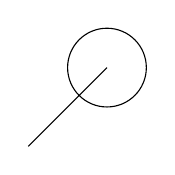
\begin{tikzpicture}\draw (0,0) -- (1,1) circle (0.5);\end{tikzpicture}
\caption{A tikz drawing.}
\end{figure}
Water is \ce{H2O}. An unknown macro \foobar{x} and math $\badmacro{y}$ here.
\begin{thebibliography}{1}\bibitem{k} K. Author, Title, 2020.\end{thebibliography}
\end{document}
